\documentclass[cic,tc,english]{iiufrgs}

% Use unicode
\usepackage[utf8]{inputenc}

% Necessário para incluir figuras
\usepackage{graphicx}
\graphicspath{{figs/}}
\DeclareGraphicsExtensions{.pdf,.jpg,.png}

\usepackage{times}            % pacote para usar fonte Adobe Times
% \usepackage{palatino}
% \usepackage{mathptmx}       % p/ usar fonte Adobe Times nas fórmulas

\usepackage[alf,abnt-emphasize=bf]{abntex2cite}

%%%%%%%%%%%%%%%%%%%%%%%%%%%%%%%%%%%%%%%%%%%%%%%%%%%%%%%%%%%%%%%%%%%%
%%%%%%%%%%%%%%%%%%%%%%%%%%%%%%%%%%%%%%%%%%%%%%%%%%%%%%%%%%%%%%%%%%%%
%
% Informações gerais
%
\title{An Interactive Tool for Learning and Exploring Shader Programming}
\author{Baptista}{Khin Emmanuel Rodrigues}
\advisor[Prof.~Dr.]{Oliveira}{Manuel Menezes de}

\date{julho}{2018}
\location{Porto Alegre}{RS}

% itens individuais da nominata podem ser redefinidos com os comandos
% abaixo:
% \renewcommand{\nominataReit}{Prof\textsuperscript{a}.~Wrana Maria Panizzi}
% \renewcommand{\nominataReitname}{Reitora}
% \renewcommand{\nominataPRE}{Prof.~Jos{\'e} Carlos Ferraz Hennemann}
% \renewcommand{\nominataPREname}{Pr{\'o}-Reitor de Ensino}
% \renewcommand{\nominataPRAPG}{Prof\textsuperscript{a}.~Joc{\'e}lia Grazia}
% \renewcommand{\nominataPRAPGname}{Pr{\'o}-Reitora Adjunta de P{\'o}s-Gradua{\c{c}}{\~a}o}
% \renewcommand{\nominataDir}{Prof.~Philippe Olivier Alexandre Navaux}
% \renewcommand{\nominataDirname}{Diretor do Instituto de Inform{\'a}tica}
% \renewcommand{\nominataCoord}{Prof.~Carlos Alberto Heuser}
% \renewcommand{\nominataCoordname}{Coordenador do PPGC}
% \renewcommand{\nominataBibchefe}{Beatriz Regina Bastos Haro}
% \renewcommand{\nominataBibchefename}{Bibliotec{\'a}ria-chefe do Instituto de Inform{\'a}tica}
% \renewcommand{\nominataChefeINA}{Prof.~Jos{\'e} Valdeni de Lima}
% \renewcommand{\nominataChefeINAname}{Chefe do \deptINA}
% \renewcommand{\nominataChefeINT}{Prof.~Leila Ribeiro}
% \renewcommand{\nominataChefeINTname}{Chefe do \deptINT}

% A seguir são apresentados comandos específicos para alguns
% tipos de documentos.

% Relatório de Pesquisa [rp]:
% \rp{123}             % numero do rp
% \financ{CNPq, CAPES} % orgaos financiadores

% Trabalho Individual [ti]:
% \ti{123}     % numero do TI
% \ti[II]{456} % no caso de ser o segundo TI

% Monografias de Especialização [espec]:
% \espec{Redes e Sistemas Distribuídos}      % nome do curso
% \coord[Profa.~Dra.]{Weber}{Taisy da Silva} % coordenador do curso
% \dept{INA}                                 % departamento relacionado

%
% palavras-chave
% iniciar todas com letras minúsculas, exceto no caso de abreviaturas
%
\keyword{formatação eletrônica de documentos}
\keyword{\LaTeX}
\keyword{ABNT}
\keyword{UFRGS}

%\settowidth{\seclen}{1.10~}

%%%%%%%%%%%%%%%%%%%%%%%%%%%%%%%%%%%%%%%%%%%%%%%%%%%%%%%%%%%%%%%%%%%%
%%%%%%%%%%%%%%%%%%%%%%%%%%%%%%%%%%%%%%%%%%%%%%%%%%%%%%%%%%%%%%%%%%%%

\begin{document}

% folha de rosto
% às vezes é necessário redefinir algum comando logo antes de produzir a folha de rosto:
% \renewcommand{\coordname}{Coordenadora do Curso}
\maketitle

% dedicatoria
% \clearpage
% \begin{flushright}
%     \mbox{}\vfill
%     {\sffamily\itshape
%       ``If I have seen farther than others,\\
%       it is because I stood on the shoulders of giants.''\\}
%     --- \textsc{Sir~Isaac Newton}
% \end{flushright}

% agradecimentos
%\chapter*{Agradecimentos}
%Agradeço ao \LaTeX\ por não ter vírus de macro\ldots


%%%%%%%%%%%%%%%%%%%%%%%%%%%%%%%%%%%%%%%%%%%%%%%%%%%%%%%%%%%%%%%%%%%%
%%%%%%%%%%%%%%%%%%%%%%%%%%%%%%%%%%%%%%%%%%%%%%%%%%%%%%%%%%%%%%%%%%%%

% resumo na língua do documento
% As a general rule, do not put math, special symbols or citations
% in the abstract
\begin{abstract}
    Learning shader programming often requires the novice to create an entire host application, having to manually load polygonal models and textures, and to deal with graphics API details. This process can be quite discouraging, deviating one's attention from actual shader programming to the development of application infrastructure. To alleviate this load, shader development environments have been created by GPU manufacturers, such as NVIDIA's FX Composer and AMD's RenderMonkey, but both have long been discontinued, not supporting modern shading languages. Available on-line resources, like Shadertoy and Shdr, can be valuable tools in assisting the learning of shader programming, but are often difficult to use, have limited feature sets, and/or lack proper documentation to get beginners started. We present a complete environment for learning and exploring shader programming using GLSL. Our environment, developed using Vulkan, can suit the needs of both beginners and advanced users. Its user-friendly interface allows one to effortlessly load 3D models and images and modify variables and textures, applying the changes in real time.
\end{abstract}


% resumo na outra língua
% como parametros devem ser passados o titulo e as palavras-chave na outra língua, separadas por vírgulas

\begin{englishabstract}
{ Uma Ferramenta Interativa para o Aprendizado e Exploração de Programação de Shaders }
{ Programação de shaders. GLSL. vulkan. computação gráfica }

    O aprendizado de programação de shaders comumente requer que o novato crie uma aplicação hospedeira completa, carregando manualmente modelos poligonais e texturas e lidando com detalhes da API gráfica. Esse processo pode ser bastante desencorajador, desviando a atenção da programação de shaders para o desenvolvimento da infraestrutura da aplicação. Para aliviar esse trabalho, ambientes de desenvolvimento de shaders foram criados por fabricantes de GPUs, como o FX Composer da NVIDIA e o RenderMonkey da AMD, mas ambos foram descontinuados há bastante tempo, e não oferecem suporte a linguagens modernas de shading. Recursos disponíveis on-line, como Shadertoy e Shdr, podem ser ferramentas valiosas para ajudar no aprendizado de programação de shaders, mas costumam ser difíceis de utilizar, possuem um conjunto de funcionalidades limitado e/ou não oferecem documentação adequada para iniciantes. Nós apresentamos um ambiente completo para o aprendizado e exploração de programação de shaders utilizando GLSL. Nosso ambiente, desenvolvido usando Vulkan, é capaz de suprir as necessidades de usuários iniciantes bem como experientes. Sua interface amigável permite que o usuário carregue modelos 3D e imagens sem dificuldade, além de modificar variáveis e texturas, aplicando as mudanças em tempo real.

\end{englishabstract}


% lista de figuras
\listoffigures

% lista de tabelas
\listoftables

% lista de abreviaturas e siglas
% o parametro deve ser a abreviatura mais longa
\begin{listofabbrv}{OpenGL}
    \item[GPU] Graphics Processing Unit
    \item[OpenGL] Open Graphics Library
    \item[GLSL] OpenGL Shading Language
    \item[HLSL] High-Level Shading Language
    \item[SPIR] Standard Portable Intermediate Representation
\end{listofabbrv}

% idem para a lista de símbolos
% \begin{listofsymbols}{$\alpha\beta\pi\omega$}
%     \item[$\sum{\frac{a}{b}}$] Somatório do produtório
%     \item[$\alpha\beta\pi\omega$] Fator de inconstância do resultado
% \end{listofsymbols}

% sumario
\tableofcontents

%%%%%%%%%%%%%%%%%%%%%%%%%%%%%%%%%%%%%%%%%%%%%%%%%%%%%%%%%%%%%%%%%%%%
%%%%%%%%%%%%%%%%%%%%%%%%%%%%%%%%%%%%%%%%%%%%%%%%%%%%%%%%%%%%%%%%%%%%

\chapter{Introduction}

Shader programming is an essential part of modern computer graphics. However, in order to write her/his first shader program, one is often faced with the need to write an entire host application that will supply data for the shader. This includes establishing associations between variables from the host program and from the shader, loading polygonal models, setting parameters, initializing textures, etc.  
All this can be quite discouraging for a novice, deviating one's attention from actual shader programming to the development of application infrastructure.

To make it easier for newcomers, we have built an application that provides a complete environment for shader programming. With this tool, one will be able to write shaders without having to worry about such infrastructure details. By being able to focus on the shaders themselves and get results faster, we hope to encourage more students to learn computer graphics. Developing such a tool also had another important personal goal: serve as an opportunity for learning Vulkan, a modern graphics API.

Our application allows students to easily prototype shaders using an integrated source code editor, and to view the results in real time in the visualization window, which can include any objects the user wants to add, including custom meshes that can be imported. While implementing this tool, we were able to understand the inner workings of Vulkan, an API which is growing fast and becoming more present in the industry of computer graphics.

This thesis is organized as follows: Chapter 2 presents the reader with a base knowledge about computer graphics and how the modern graphics applications perform their functions, as well as introduces Godot Engine, the tool used to create our application. Chapter 3 introduces important details of the Vulkan API and how it differs from OpenGL. Chapter 4 describes the methods applied in the implementation of our tool, the architecture of our application and how to use it from a user perspective. Chapter 5 presents the results we were able to obtain using our solution. Chapter 6 concludes this work, presenting our view of the tool developed. Chapter 7 discusses how our application could be improved in the future.

\section{Related work}
As we mentioned, many attempts were made to create a proper development environment for shaders.

\textbf{FX Composer}, developed by NVIDIA, featured an integrated source code editor, a scene visualizer which could use DirectX 10, DirectX 9 or OpenGL, widgets for editing parameters, particle systems, material manager, material preview and much more \cite{fxcomposer}. My personal experience with FX Composer confirms the software has not been updated since 2008 \cite{fxcomposer_release_notes}: many usability issues and bugs were encountered while in class, such as debug messages pointing to errors that were not from the user code but from the software architecture. This in part motivated me to create this work.

\textbf{RenderMonkey}, developed by AMD, aimed to provide tools for both programmers and artists. It featured a complete shader source editor and preview window, but also a workspace specific for artists, where much of the shader programming was hidden from the user, widgets used to adjust parameter values. It presented support for HLSL, GLSL and GLES shading languages \cite{rendermonkey}. The latest version of the software was released in 2008 \cite{rendermonkey_release_notes} and AMD's website no longer displays any information about the software or that it ever existed.


\textcolor{red}{Antes da secao de Background voce deve apresentar uma secao de trabalhos relacionados (Related Work).}

\chapter{Background}

%\textcolor{red}{As duas proximas secoes devem ser convertidas em um glossario. Inicie esta secao fazendo uma breve apresentacao sobre o pipeline grafico, ate que voce chegue ao conceito de shaders. Depois inclua uma secao explicando o que sao shaders. Depois disso, voce apresentara a secao sobre Vulcan. Note que esta eh uma secao de background para os dois temas centrais do trabalho: shader programming e Vulkan.}

In this chapter, we will introduce important concepts of computer graphics which the reader is expected to be familiar with. Concepts from linear algebra like vector maths, matrix operations and geometric transformations are presumed to be understood.

\section{Graphics pipeline}
In the field of computer graphics, \textbf{graphics pipeline} is the name of the algorithm used to generate 2D images out of 3D geometric information. Figure \ref{fig:graphics_pipeline} shows a diagram describing the stages of the graphics pipeline. Each stage of the pipeline is responsible for a specific operation; the output of each stage is passed to the next stage to be used as input.

The function performed by each of the stages in the pipeline are described as follows \cite{vulkan_tutorial}:

\begin{itemize}
    \item Input assembler: Collects the raw vertex data from the vertex buffer and may also use an index buffer to repeat certain elements without having to duplicate the vertex data itself;
    \item Vertex shader: Executed for every vertex in the object, generally applies transformations to turn vertex positions from model space to screen space;
    \item Tesselation: Optional stage which subdivides geometry based on certain rules to increase mesh quality;
    \item Geometry shader: Optional stage executed for every primitive (point, line, triangle) which is able to discard or create new primitives;
    \item Rasterization: Breaks down the primitives into fragments, which are the pixel elements that will make up the rendered image. Fragments located outside the screen space are discarded, and vertex data is interpolated across the fragments;
    \item Fragment shader: Invoked for every fragment, determines its color based on the interpolated vertex data outputted by the raterization stage;
    \item Color blending: Applies operations to mix different fragments that map to the same pixel in the resulting image, usually based upon transparency.
\end{itemize}

\begin{figure}[h]
    \caption{Graphics pipeline}
    \begin{center}
        \includegraphics[width = 7cm]{"vulkan_pipeline"}
    \end{center}
    \label{fig:graphics_pipeline}
    \legend{Source: \cite{vulkan_tutorial}}
\end{figure}

Certain stages can only be controlled by changing their parameters, but the function performed is always the same. These are known as \textit{fixed function stages} and are the ones in green in Figure \ref{fig:graphics_pipeline}.

The other stages, in orange, are known as the \textit{programmable stages}, which means developers can upload source code to the graphics card to apply exactly the operations they intended for that stage.

From the programmable stages, tesselation shaders and geometry shaders are optional, meaning that their functions can be skipped and the pipeline can still work properly. On the other hand, the \textit{vertex shader} and the \textit{fragment shader} are required from the developer and the graphics pipeline cannot function without them.

Shaders always receive data from the previous stage of the pipeline, but they can also define additional parameters to be used in their computations. These parameters are called \textit{uniform variables}. Uniform variables can have their values changed from one frame to the next, but for every time the shader is executed in a frame, the uniform variable will have the exact same value. These variables can be used to, for example, tell the shader where the lights are located in the scene, or provide an image to be used as texture. These values must be supplied from the host application, which manages the graphics pipeline.

The following code represents the basic operation of a vertex shader:

\begin{verbatim}
    uniform mat4 modelViewProjection;
    in vec4 position;
    out vec4 clip_position;
    void main() {
        clip_position = modelViewProjection * position;
    }
\end{verbatim}

The first line defines a uniform variable which is a matrix that will transform vertices from local space to clipping space (a normalized space required by the next stages of the pipeline). This matrix accumulates model, view and the projection matrices. The model matrix applies rotation, scale and translation to the object's vertices, transforming them from local space to world space. The view matrix transforms the vertex positions from world space to view space, where the camera is at the origin. Finally, the projection matrix will deform the geometry to apply perspective or orthogonal projections.

The second line describes the vertex attribute that the vertex shader expects to receive from the input assembler. This simple example expects just the vertex position, but it could require other attributes, such as normal vectors or texture coordinates.

The third line describes the output of this shader. Since it is a vertex shader, the vertex position in clip space is required to be an output. Other output variables can be defined, and these variables will be interpolated by the rasterizer and delivered to the fragment shader.

The following code represents the basic operation of a fragment shader:

\begin{verbatim}
    uniform vec4 frag_color;
    out vec4 final_color;
    void main() {
        final_color = frag_color;
    }
\end{verbatim}

The purpose of the fragment shader is to output the color of the fragment. This sample code does just that: a uniform variable is used as color for the fragment. The \texttt{vec4} variable type can be used to represent colors because it holds four floating point values, which are interpreted as red, green, blue and alpha channels.

\section{Graphics APIs}
As we have mentioned, graphics applications require a host application to manage its operation. The means used to do that is through a graphics API. Graphics APIs are a set of routines implemented by graphics cards manufacturers that allows developers to control the hardware. Examples of graphics APIs include Direct3D, OpenGL, Metal and Vulkan. Each API defines their own set of methods and how they are used, and it is up for hardware manufacturers to support the APIs. Some APIs, such as Direct3D and Metal, are proprietary to enterprises (namely, Microsoft and Apple, respectively) and can only be used on their platforms. Others, like OpenGL and Vulkan, are open standards, both provided by the Khronos group, an industry consortium. This work uses the Vulkan API to fulfill a personal goal of creating a functional piece of software using this relatively new API.

\section{Vulkan}
Vulkan is a new generation graphics and compute API that provides high-efficiency, cross-platform access to modern GPUs used in a wide variety of devices from PCs and consoles to mobile phones and embedded platforms \cite{vulkan}.

\subsection{Validation layers}
The Vulkan API is designed around the idea of minimal driver overhead and one of the manifestations of that goal is that there is very limited error checking in the API by default. Even mistakes as simple as setting enumerations to incorrect values or passing null pointers to required parameters are generally not explicitly handled and will simply result in crashes or undefined behavior \cite{vulkan_tutorial}. Vulkan comes with a set of validation and debug layers as part of the Vulkan SDK. When any subset of these layers are enabled they insert themselves automatically into the call-chain of every Vulkan API call issued by the application to perform their job. Validation layers can also report warnings about potential incorrect or dangerous use of the API, and are even capable of reporting performance warnings that allow developers to identify places where the API is used correctly but not used in the most efficient way \cite{vulkan_validation_layers}.

\subsection{Memory management}
While OpenGL drivers manage memory allocations transparently to the programmer, Vulkan not only allows but also requires that programmers allocate device memory (in our case, GPU memory) and bind the memory to the resources used in the application. While this may increase the application's performance if the programmer takes advantage of it, it also requires the programmer to manually manage buffer alignments and aliasing.  The recommended way of allocating memory and creating buffers is described in Figure \ref{fig:vulkan_mem_alloc}.

\begin{figure}[ht]
    \centering
    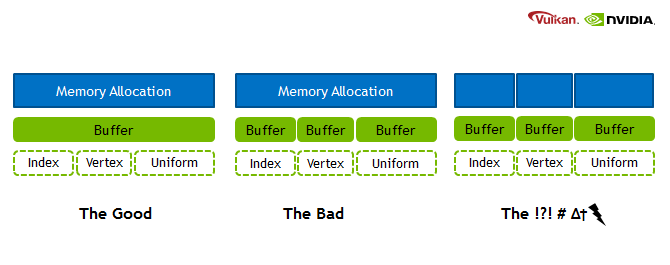
\includegraphics[width = 15cm]{figs/vulkan_memory_strategy.png}
    \caption{Vulkan memory allocation strategies}
    \label{fig:vulkan_mem_alloc}
\end{figure}

This diagram illustrates three memory allocation strategies \cite{vulkan_mem_mgmt}.
The rightmost is the naive approach: for each buffer is performed a "dedicated" memory allocation. This approach is the easiest to implement, since every object allocates, binds and frees their own memory, without taking into account other objects created. It is also the least optimized approach, given that this most likely will not be cache-friendly. It is also important to note that Vulkan devices have a maximum number of memory allocations that can exist simultaneously;
The approach shown in the middle, captioned "The Bad", shows a single memory allocation with various buffers bound to it. This approach is more cache-friendly than the previous one, but it requires the programmer to deal with memory aliasing, offsets and buffer alignments;
The leftmost, captioned as "The Good", is the recommended approach. It represents a single memory allocation bound to a single buffer, with different data loaded to different areas of the buffer. This approach is the most cache-friendly and the most optimized for performance in highly dynamic scenes, but also the most difficult to implement. This setup is possible thanks to Vulkan low-level control of offsets even inside a single buffer, allowing the developer to define "virtual buffers".

In this work, our goal was to build a simple scene with few objects, for the purposes of visualization only. For this reason, we opted to use the naive approach. Implementing a memory management module would not perceivably impact on the performance of the application.

\subsection{Compiling shaders}
Up until OpenGL 4.6, application had to be compile shader source code at run-time, passing a string of high-level source code to the graphics driver. While this allowed the application to run on different hardware, this also forced each GPU manufacturer to provide a GLSL compiler with the device driver, making it difficult for vendors to update and support new versions of the API in their drivers.

\subsubsection{SPIR-V}
The "Standard Portable Intermediate Representation" version "V" (as in "Vulkan") is a binary representation of shader code which device drivers can parse more easily. Application developers, having their shaders written, must compile them into SPIR-V format before loading them in their applications. This contributes for quicker development of device drivers. Support for SPIR-V shaders is included in OpenGL 4.6 and Vulkan 1.0.


% WILL GO TO A "GLOSSARY" OF SORTS
%\section{Rendering}
According to \cite{shirley_fcg:2002}, \emph{rendering} is a term inherited from art and deals with the creation of shaded images from 3D computer models.
%\section{Illumination models}

%\section{Shading models}
%\subsection{Phong shading model}

\section{Shading languages}
Programming languages designed for computer graphics, which are used to define shaders, implementing an illumination model. Various shading languages exist:

\begin{itemize}
    \item CG: \emph{C for Graphics}, developed by NVidia in collaboration with Microsoft, it has been deprecated since 2012;
    \item HLSL: \emph{High-Level Shader Language}, used with DirectX 9 and higher;
    \item GLSL: \emph{OpenGL Shading Language}, used with OpenGL.
\end{itemize}

In this work, all the shader code was written in GLSL. We will not be covering the GLSL language specifics; there are entire books about it, and it goes beyond the scope of this text.



\chapter{Method}

\section{Architecture}
In this work, the most important decision of the architecture was the choice of using Vulkan for the graphics API. Using Vulkan has been a learning process, and the architecture chosen is a reflection of it.

\subsection{Vulkan Application Module}
Vulkan is a low-level API and, as such, requires developers to setup a large amount of objects and configurations before displaying anything on screen. This module is responsible for creating these objects required for rendering.

\subsubsection{Vulkan Instance}
There is no global state in Vulkan and all per-application state is stored in a VkInstance object. Creating a VkInstance object initializes the Vulkan library and allows the application to pass information about itself to the implementation \cite{vulkan_docs}. Applications can even define and manage multiple instances if they so desire.

In order to initialize a Vulkan instance object, we first need to create a VkApplicationInfo structure object, which will describe our application for the driver. This structure hold the name and version of the application, and also the name and version of the engine used. This data is technically optional, but it may provide some useful information to the driver to optimize for our specific application, for example because it uses a well-known graphics engine with certain special behavior \cite{vulkan_tutorial}. Unlike the VkApplicationInfo, the VkInstanceCreateInfo structure object is not optional. It describes the instance extensions and debug layers we want to enable in our application. To make sure our application can be executed, we can check the available extensions with the function vkEnumerateInstanceExtensionProperties to compare against our required extensions. In our application, we are using GLFW for window management, which provides the glfwGetRequiredInstanceExtensions function \cite{glfw_vulkan} to query the required functions for surface creation on any platform supported by the library.

During the Vulkan instance object creation we can also specify validation layers to be enabled. Available validation layers can be queried with the vkEnumerateInstanceLayerProperties function. The Vulkan SDK provides a standard validation layer, "VK\_LAYER\_LUNARG\_standard\_validation", which implicitly enables a range of useful diagnostic layers. In order to receive the debug messages from the validation layers, however, the application must also enable the "VK\_EXT\_debug\_report" extension, which will allow the developer to setup a callback function that will be called whenever a debug message is issued by the validation layers. To setup the debug callback function, the developer has to get a pointer to the vkCreateDebugReportCallbackEXT, which is an extension function and therefore not included in the base API, using the vkGetInstanceProcAddr function.

\subsubsection{Physical Device}
The function vkEnumeratePhysicalDevices returns a list of available Vulkan devices installed in the system. Basic device properties like the name, type and supported Vulkan version can be queried using vkGetPhysicalDeviceProperties. The support for optional features like texture compression, 64 bit floats and multi viewport rendering can be queried using vkGetPhysicalDeviceFeatures. Device features must be enabled before they are used by the application.

Almost every operation in Vulkan, from drawing to uploading textures, requires commands to be submitted to a queue. A queue belongs to a \emph{queue family}, and each queue family supports certain types of commands. For a rendering application like ours, we need a queue able to render graphics, and another queue for presentation (displaying images in the window). These queues could be the same, if the physical device presents a single queue with both graphics and presentation capabilities. To query queue families, there is a vkGetPhysicalDeviceQueueFamilyProperties function.

With a list of the available devices, their features and queue families, we can select a VkPhysicalDevice and create a logical device to interface with it.

\subsubsection{Device}
The logical device creation process is similar to the instance creation process and describes the features we want to use in our application. We also need to specify which queues to create from the queue families that are available. 

The function vkCreateDevice takes the physical device we selected and a VkDeviceCreateInfo object as arguments. The latter describes which physical device features we want to enable from our selected physical device. We must also specify the queues we want to create, indicating the queue family index and amount of queues we want to create from each family. After the device is created, the application can call the vkGetDeviceQueue function to get the VkQueue objects to which commands will be passed into.

\subsubsection{Window Surface}



\subsection{Shader Module}
A Shader object represents one stage of the programmable pipeline stages. This module has a type indication, either vertex or fragment, and is capable of loading GLSL source files and compiling them into SPIR-V binary using the ShaderC library, developed by Google. The compiled code is then enclosed by a 'VkShaderModule' object which will be used in a material's graphics pipeline.

The type of the shader is inferred when a GLSL shader file is loaded based on the extension of the shader file, '.vert' for a vertex shader and '.frag' for a fragment shader.

This module also provides ways to check the compilation status and get any compilation error messages.


\subsection{Material Module}
A Material is a combination of a vertex and a fragment shader, plus the values of the uniform variables defined in those shaders. It is responsible for the creation of the Vulkan graphics pipeline object, based on the shaders loaded into it and other configuration values.

\subsubsection{Shader Parsing}
The shaders added to the material will have their SPIR-V code parsed by the \emph{SPIRV Cross} library. Our application will use this data to load the appropriate vertex attributes, uniform objects and sampler objects used by the shaders.

Shaders define which vertex attributes will be used as input, and uniform variables can serve as parameters for the material. All vertex attributes must be recognized by our application, following the defined names and types defined in table \ref{tab:vertex_attributes}. The user can also query the application for certain uniform variables, following the names and types defined in Table \ref{tab:uniform_variables}.

\begin{table}[h]
    \centering
    \caption{Recognized vertex attributes}
    \begin{tabular}{|c|c|p{6cm}|}
    \hline
        \textit{Type} & \textit{Name} & \textit{Description} \\
        \hline \hline
        vec3 or vec4 & \texttt{position} & Vertex position \\
        vec3 or vec4 & \texttt{normal} & Normal vector of the surface \\
        vec3 or vec4 & \texttt{tangent} & Tangent vector to the surface \\
        vec2 & \texttt{uv} & Texture coordinate \\
        \hline
    \end{tabular}
    \label{tab:vertex_attributes}
\end{table}

If the \texttt{position} attribute is a vec4, the fourth component will be set to one; If the \texttt{normal} is a vec4, the fourth component will be set to zero; If the \texttt{tangent} is a vec4, the fourth component will be either set do 1 or -1, indicating the direction pointed by the binormal vector, used in normal mapping.

\begin{table}[h]
    \centering
    \caption{Recognized uniform variables}
    \begin{tabular}{|c|c|p{6cm}|}
        \hline
        \textit{Type} & \textit{Name} & \textit{Description} \\
        \hline
        \hline
        mat4 & \texttt{model} & Model matrix \\
        mat4 & \texttt{view} & View matrix \\
        mat4 & \texttt{projection} & Projection matrix \\
        mat4 & \texttt{modelView} & Model-View matrix \\
        mat4 & \texttt{modelViewProjection} & Model-View-Projection matrix \\
        mat4 & \texttt{modelInverse} & Model matrix inverse \\
        mat4 & \texttt{viewInverse} & View matrix inverse \\
        mat4 & \texttt{projectionInverse} & Projection matrix inverse \\
        mat4 & \texttt{modelViewInverse} & Model-View matrix inverse \\
        mat4 & \texttt{modelViewProjectionInverse} & Model-View-Projection matrix inverse \\
        mat3 & \texttt{normalMatrix} & Matrix to transform the normal vectors of the object; Corresponds to the inverse transposed 3x3 model-view submatrix \\
        \hline
    \end{tabular}
    \label{tab:uniform_variables}
\end{table}

Note that the normal matrix is a 3x3 matrix, unlike the other ones. This is because the correct matrix to transform the normal vector is the transpose of the inverse of the 3x3 submatrix from the model view matrix \cite{normal_matrix}.

The shader code can also define arbitrary uniform variables, which will be initialized to a default value and exposed in the control window so the user can change the values manually. Numeric values are initialized to 1 to avoid division by zero. Image samplers defined in code will be initialized to a white texture.

\subsubsection{Descriptor set layout and descriptor pool}
After the shaders are parsed, the Material module will create the descriptor set layout object ('VkDescriptorSetLayout') and descriptor pool. In our case, every uniform buffer object and image sampler is available in all graphics stages (vertex and fragment). For this reason, the shaders must declare the binding of each uniform buffer object and image sampler used in GLSL code, and the binding numbers cannot be reused. This is done in GLSL by using the layout qualifier in the declaration of the uniforms.

For our application, the size of the descriptor pool translates into how many different objects can have the same material applied at a given time.


\subsection{Geometry Module}
The geometry module represents an object in the scene. It holds all the vertices attributes (vertex position, normal, tangent, texture coordinates and indices, if available); a transformation, which defines the rotation, scale and translation applied to the object; and a reference to a material object which will be used to render the geometry in the scene.

\subsubsection{Vertex, Index and Uniform Buffers}
When an object is added to the scene, it must be filled with vertex data and then a material has to be assigned to the material. Then, the object will get a list of the required vertex attributes from the material, and create the vertex buffer accordingly. If the vertex attributes include index data, the index buffer is created, too. Then, the uniform buffers are created, based on the uniform buffer objects in the material assigned.

\subsubsection{Descriptor Sets}
For the uniform buffer to be passed to the shaders, we need to allocate a descriptor set from the pool defined in the material assigned to this geometry. We need to do this because the descriptor layout in the material is just a description of what types of descriptors can be bound, but no uniform buffer has been referenced yet. The descriptor set specifies a buffer to be bound in the uniform buffer descriptor.

\subsubsection{Recording Drawing Commands}
Since all drawing operations are recorded in advance in Vulkan, this module also provides a method for recording the drawing commands in a command buffer previously initialized.

\subsubsection{Updating Uniform Buffers}
The function to update uniform buffers is called by the Vulkan application module, and expects a structures containing certain uniform values that are not dependent on the object, such as the camera's view and projection matrices. The other matrices are calculated and loaded into the appropriate buffers.

The material can define arbitrary uniform variables, and those must be updated as well. The material holds an array of dictionaries that describe each of the user-defined variables, their types, sizes, bindings, offsets and values. With this information, our application is able to load the variable value into the correct buffer in the correct offset.


\subsection{Texture Module}
The texture module handles the passage of image data for the shaders. This means creating an image, allocating device memory for the image, creating the image view and the sampler.

Image files are loaded by Godot, the engine used to create the user interface, and their data is passed to the texture module. Our application then has to pass this data into the device memory bound to the image. However, there is no way to write directly to the image memory, which forces us to use a \textit{staging buffer}. The staging buffer can be mapped to CPU memory and accessed by our application. In order to transfer this data to the image, the image must have its layout transitioned to optimal for transfer destination. This is done using a single time command buffer, which is allocated, recorded, executed and freed, sequentially. Single time command buffers are managed by the Vulkan application module. Once the image is ready to receive a data transfer and the staging buffer is loaded, we can use another single time command buffer to copy the buffer contents into the image. After this transfer is complete, the image must be transitioned again to a layout optimal for shader read only. Then, the staging buffer can be destroyed, and the device memory can be freed.


\subsection{Camera Module}
The camera module represents a virtual camera. It has a position, target and up vectors for reference and an angle for the field of view of the projection. This module provides the view and projection matrices used to transform the objects in the shaders. It also presents methods for moving and turning, used by the Vulkan application module.



\section{User Interface}
In this section we will describe how our application works from a user perspective, explaining the different panels, their responsibilities and how to use them.

\begin{figure}[ht]
    \caption{Application control window}
    \begin{center}
        \includegraphics[width = 15cm]{"editor/window"}
    \end{center}
    \label{fig:window}
    \legend{Source: the author}
\end{figure}


%%%%%%%%%%%%%%%%%%%%%%%%%%%%%%%%%%%%%%%%%%%%%%%%%%
\subsection{Materials and Shaders}
When the application is first executed, a default material is loaded. This is a simple unshaded material that will be assigned to new objects when they are created. This material does not require the geometry to have any any attributes other than position, which ensures this material can be applied to any loaded mesh.

The \textit{create button} (labeled with a plus sign) allows the user to load shaders and create a new material via the \textit{create material} popup window (Figure \ref{fig:create-material}). The material name must be unique and the vertex and fragment shaders source files must have a ".vert" and ".frag" extension, respectively. When the material is created, the contents of the shader files are loaded in the shader editor (Figure \ref{fig:shader-editor}). At this point, the material is not ready for usage yet.

\begin{figure}[h]
    \caption{Create material popup window}
    \begin{center}
        \includegraphics[width = 10cm]{"editor/create-material"}
    \end{center}
    \label{fig:create-material}
    \legend{Source: the author}
\end{figure}

\begin{figure}
    \caption{Shader editor}
    \begin{center}
        \includegraphics[width = 10cm]{"editor/shader-editor"}
    \end{center}
    \label{fig:shader-editor}
    \legend{Source: the author}
\end{figure}

The GLSL source code for the vertex and fragment shaders can be altered in the shader editor, which features syntax highlighting, line numbers, highlight selected word occurrences and a shader compilation status bar.

In order to compile the shaders and setup the material, the user can click on the execute button in the material list panel (the button with the "play" icon). The shaders are then compiled and loaded in the material. If the compilation is unsuccessful, the status bar, right under the fragment shader editor, displays the error messages. When the compilation succeeds, the uniforms defined in the shaders' source code are exposed in the material parameters panel (Figure \ref{fig:uniform-editor}).

\begin{figure}
    \caption{Uniform editor}
    \begin{center}
        \includegraphics[width = 10cm]{"editor/uniform-editor"}
    \end{center}
    \label{fig:uniform-editor}
    \legend{Source: the author}
\end{figure}

The editor creates appropriate widgets for each uniform variable defined in the shaders based on their types. Supported types are described in Table \ref{tab:uniform_types}.

\begin{table}
    \centering
    \caption{Recognized types for uniform variables}
    \begin{tabular}{|c|p{10cm}|}
        \hline
        Type name & Widget created \\
        \hline \hline
        \texttt{int} & Single numerical input widget. Accepts values from -10000 to 10000. Fractions are rounded. \\ \hline
        \texttt{uint} & Single numeric input widget. Accepts values between 0 and 10000. Fractions are rounded. \\ \hline
        \texttt{float} & Single numeric input field. Accepts values between -10000.0 and 10000.0. Uses 2 decimal digits. \\ \hline
        \texttt{ivec2} & Two numerical input widgets. Each widget follows the same input rules as \texttt{int}. \\ \hline
        \texttt{uvec2} & Two numerical input widgets. Each widget follows the same input rules as \texttt{uint}. \\ \hline
        \texttt{vec2} & Two numerical input widgets. Each widget follows the same input rules as \texttt{float}. \\ \hline
        \texttt{ivec3} & Three numerical input widgets. Each widget follows the same input rules as \texttt{int}. \\ \hline
        \texttt{uvec3} & Three numerical input widgets. Each widget follows the same input rules as \texttt{uint}. \\ \hline
        \texttt{vec3} & Three numerical input widgets. Each widget follows the same input rules as \texttt{float}. \\ \hline
        \texttt{vec4} & Color picker widget \\
        \hline
    \end{tabular}
    \label{tab:uniform_types}
\end{table}

%%%%%%%%%%%%%%%%%%%%%%%%%%%%%%%%%%%%%%%%%%%%%%%%%%
\subsection{Objects}

The plus button on the objects panel allows the user to create a new object, selecting a primitive geometry from a list or loading a custom mesh file (in Wavefront ".obj" format). The geometry primitives provided are: capsule, cube, cylinder, plane, prism and sphere.

Newly created objects are given a name based on their shape (if the object is a primitive) or their file name (if it was created from a mesh file), and their creation order. New objects are assigned the default material upon creation, and instantly appear in the scene (Figure \ref{fig:default_material}).

\begin{figure}
    \caption{Dragon mesh with the default material}
    \begin{center}
        \includegraphics[width = 10cm]{"editor/default_material"}
    \end{center}
    \label{fig:default_material}
    \legend{Source: the author}
\end{figure}

When an object is selected, their transformation and currently assigned material are displayed on the inspector panel, below the material parameters panel (Figures \ref{fig:uniform-editor} and \ref{fig:inspector}). Changes made to the inspector and the material parameters take effect immediately.

\begin{figure}
    \caption{Inspector}
    \begin{center}
        \includegraphics[width = 10cm]{"editor/inspector"}
    \end{center}
    \label{fig:inspector}
    \legend{Source: the author}
\end{figure}

\begin{figure}
    \caption{Available materials appear in the inspector drop-down menu}
    \begin{center}
        \includegraphics[width = 6cm]{"editor/material_selection"}
    \end{center}
    \label{fig:material_selection}
    \legend{Source: the author}
\end{figure}

Table \ref{tab:navigation_control} shows the available commands to navigate through the scene.

\begin{table}[h]
    \centering
    \caption{Scene navigation controls}
    \begin{tabular}{|c|p{8cm}|}
        \hline
        Input & Action \\
        \hline \hline
        Mouse right click & When pressed, enables movement \\ \hline
        Mouse movement & When movement is enabled, rotates the camera around its own center, looking around \\ \hline
        'W' key & Move the camera forward, relative to its current orientation \\ \hline
        'A' key & Move the camera to the left, relative to its current orientation \\ \hline
        'S' key & Move the camera backward, relative to its current orientation \\ \hline
        'D' key & Move the camera to the right, relative to its current orientation \\
        \hline
    \end{tabular}
    \label{tab:navigation_control}
\end{table}



\section{Results}
The application allows the user to create and visualize different shaders in multiple objects, define an arbitrary number of parameters for each material and also use multiple textures to create the desired visuals.

\begin{figure*}[!t]
\centering
\subfloat[Example: Phong shading model.]{
    \includegraphics[width=3in]{"phong"}
    %\label{fig_first_case}
}
\hfil
\subfloat[Example: Normal mapping applied to a sphere.]{
    \includegraphics[width=3in]{"normal"}
    %\label{fig_second_case}
}
\hfil
\subfloat[Example: Multiple objects with different materials.]{
    \includegraphics[width=5in]{"meshes-multi-material"}
    %\label{fig_second_case}
}
\caption{Materials rendered using our application.}
%\label{fig_sim2}
\end{figure*}


\section{Conclusion}
The application we created is a tool that allows students to write shader code without having to worry about the underlying graphics API or creating the application infrastructure just to see the shaders in action. The results show we were successful in creating such tool, rendering different scenes very quickly, which shows the flexibility of this tool.

Creating this application has been a great learning exercise of the Vulkan API, and the efforts have resulted in a very interesting piece of software with a real-world use-case scenario, with lots of room to grow. Given the proper treatment, this application, which currently is presented as a proof of concept, could be really useful in classes, from fundamentals of computer graphics to advanced shader programming.


\section{Future Work}
We have some ideas as to how this project could be improved. For example, the definition of a project description file format would be of great benefice for students, allowing them to share projects between one another and the teacher; It may also be desirable to support more types of shaders, like geometry, tesselation control and tesselation evaluation shaders; Syntax higlighting in the integrated GLSL source code editor could contribute to help the students' learning;  Cubemap sampler support would also be useful to create certain effects; Adding lights as entities of the application, broadcasting their attributes to all shaders that required them, instead of having each shader add their own light parameters; Finally, removing and renaming resources (materials and objects) could improve the experience of students using the application.

The overall implementation could also benefit from more rigid software engineering guidelines in order to separate the core functionality to the interface used to communicate with the control window (using the "Model-View-Controller" model, for example).

This application could also be expanded to help students understand general computer graphics topics instead of just shader programming. This could be achieved if the Vulkan API configuration values in its various structures were exposed to the user in an organized manner, so that the student could tweak parameters of the entire graphics pipeline and see the changes in real time. Going even further, this could evolve into a tool to learn the Vulkan API specifically, if the user were given the chance to, for example, see the available physical devices, their features and extensions, being able to enable and disable each of them at will. Such tool could be really enlightening to anyone using the API for the first time.


%%%%%%%%%%%%%%%%%%%%%%%%%%%%%%%%%%%%%%%%%%%%%%%%%%%%%%%%%%%%%%%%%%%%
%%%%%%%%%%%%%%%%%%%%%%%%%%%%%%%%%%%%%%%%%%%%%%%%%%%%%%%%%%%%%%%%%%%%

% \begin{figure}[ht]
%     \caption{Descrição da Figura deve ir no topo}
%     \begin{center}
%         % Aqui vai um includegraphics , um picture environment ou qualquer
%         % outro comando necessário para incorporar o formato de imagem
%         % utilizado.
%         \begin{picture}(100,100)
%             \put(0,0){\line(0,1){100}}
%             \put(0,0){\line(1,0){100}}
%             \put(100,100){\line(0,-1){100}}
%             \put(100,100){\line(-1,0){100}}
%             \put(10,50){Uma Imagem}
%         \end{picture}
%     \end{center}
%     \label{fig:estrutura}
%     \legend{Fonte: Os Autores}
% \end{figure}

% \begin{figure}
%     \caption{Exemplo de figura importada de um arquivo e também exemplo de caption muito grande que ocupa mais de uma linha na Lista~de~Figuras}
%     \begin{center}
%         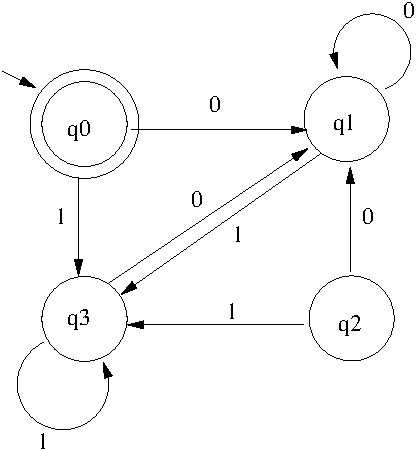
\includegraphics[width=8em]{fig}
%     \end{center}
%     \legend{Fonte: Os Autores}
%     \label{fig:ex1}
% \end{figure}

% o `[h]' abaixo é um parâmetro opcional que sugere que o LaTeX coloque a
% figura exatamente neste ponto do texto. Somente preocupe-se com esse tipo
% de formatação quando o texto estiver completamente pronto (uma frase a mais
% pode fazer o LaTeX mudar completamente de idéia sobre onde colocar as
% figuras e tabelas)

\bibliographystyle{abntex2-alf}
\bibliography{biblio}

\end{document}
